\documentclass[12pt,fleqn]{article}\usepackage{../../common}
\begin{document}
Döndürme (Rotation) - 2

Herhangi Bir Eksen (Vektör) Etrafında Dönüş

Daha öne Rodriguez yöntemi ile yaptığımız döndürme yaklaşımını bir başka
teknikle göstereceğiz. Bulmak istediğimiz $\vec{n}$ etrafında $\theta$ dönüşü
yaptıracak bir matris, yani öyle bir matris $R(\vec{n},\theta)$ arıyoruz ki bu
matrisle $\vec{v}$ vektörünü sağdan çarpınca $\vec{v}'$ elde edilecek ve bu yeni
vektör $\vec{v}$ vektörünün $\vec{n}$ etrafında $\theta$ kadar dönmüş hali
olacak,

$$
v' = v R(n,\theta)
$$

$R(n,\theta)$ matrisini türetmek için önce $v'$ vektörünü $v,n,\theta$ bazında
temsil etmeyi görelim. Ana fikir problemi $n$'ye dik olan düzlem üzerinde
çözmek, ki bu şekilde 3 boyutlu problemi 2 boyutlu bir probleme indirgemiş
oluyoruz. İndirgeme için $v$ vektörünü iki $v_\parallel$ ve $v_\perp$ vektörüne
ayıracağız, öyle ki $v = v_\parallel + v_\perp$. Sonra bu ki vektörü ayrıca
döndüreceğiz ve böylece onların toplamları da dönmüş olacak, yani $v' =
v'_\parallel + v'_\perp$. Buraya kadar gördüklerimiz Rodriguez yaklaşımına
benziyor.

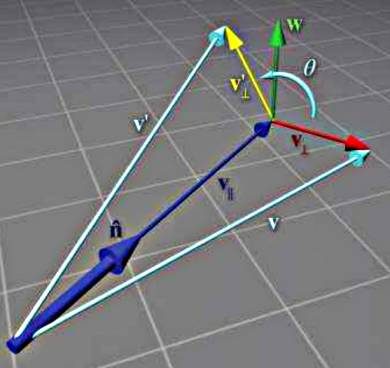
\includegraphics[width=10em]{phy_073_rot_01.jpg}

Tekniğin iyi tarafı $v_\parallel$ vektörü $n$ vektörüne paralel olduğu için $n$
etrafında dönüşten etkilenmez, o zaman sadece $v_\perp$ vektörünü döndürmek
yeterlidir, böylece $v' = v_\parallel + v'_\perp$ hesaplanabilir.

Hesap için şu adımları takip ediyoruz,

\begin{itemize}
   \item $v_\parallel$ vektörü $v$ nin $n$ ye paralel olan şeklidir, ya da
     $v$ vektörünün $n$ üzerinde yansıtılmış halidir [2], bu formülün
     $v_\parallel = (v \cdot n) n$ olduğunu biliyoruz.
   \item $v_\perp$ vektoru $v$ nin $n$ ye dik olan kismidir.
     $v = v_\parallel + v_\perp$ oldugu icin $v_\perp = v - v_\parallel$.
\end{itemize}






Kaynaklar

[1] Dunn, {\em 3D Math Primer for Graphics and Game Development}

[2] Bayramlı, {\em Lineer Cebir - Giriş}

\end{document}
